% !TEX program = xelatex

\documentclass{resume}
\usepackage{graphicx}
\usepackage{tabu}
\usepackage{multirow}
\usepackage{progressbar}
% 导入包
\usepackage{hyperref}
% 格式设置
\hypersetup{hidelinks,
	colorlinks=true,
	allcolors=black,
	pdfstartview=Fit,
	breaklinks=true}
%\usepackage{zh_CN-Adobefonts_external} % Simplified Chinese Support using external fonts (./fonts/zh_CN-Adobe/)
%\usepackage{zh_CN-Adobefonts_internal} % Simplified Chinese Support using system fonts

\begin{document}
\pagenumbering{gobble} % suppress displaying page number

{
% change Large font here
\Large{
  \begin{tabu}{ c l r }
   \multirow{4}{1in}{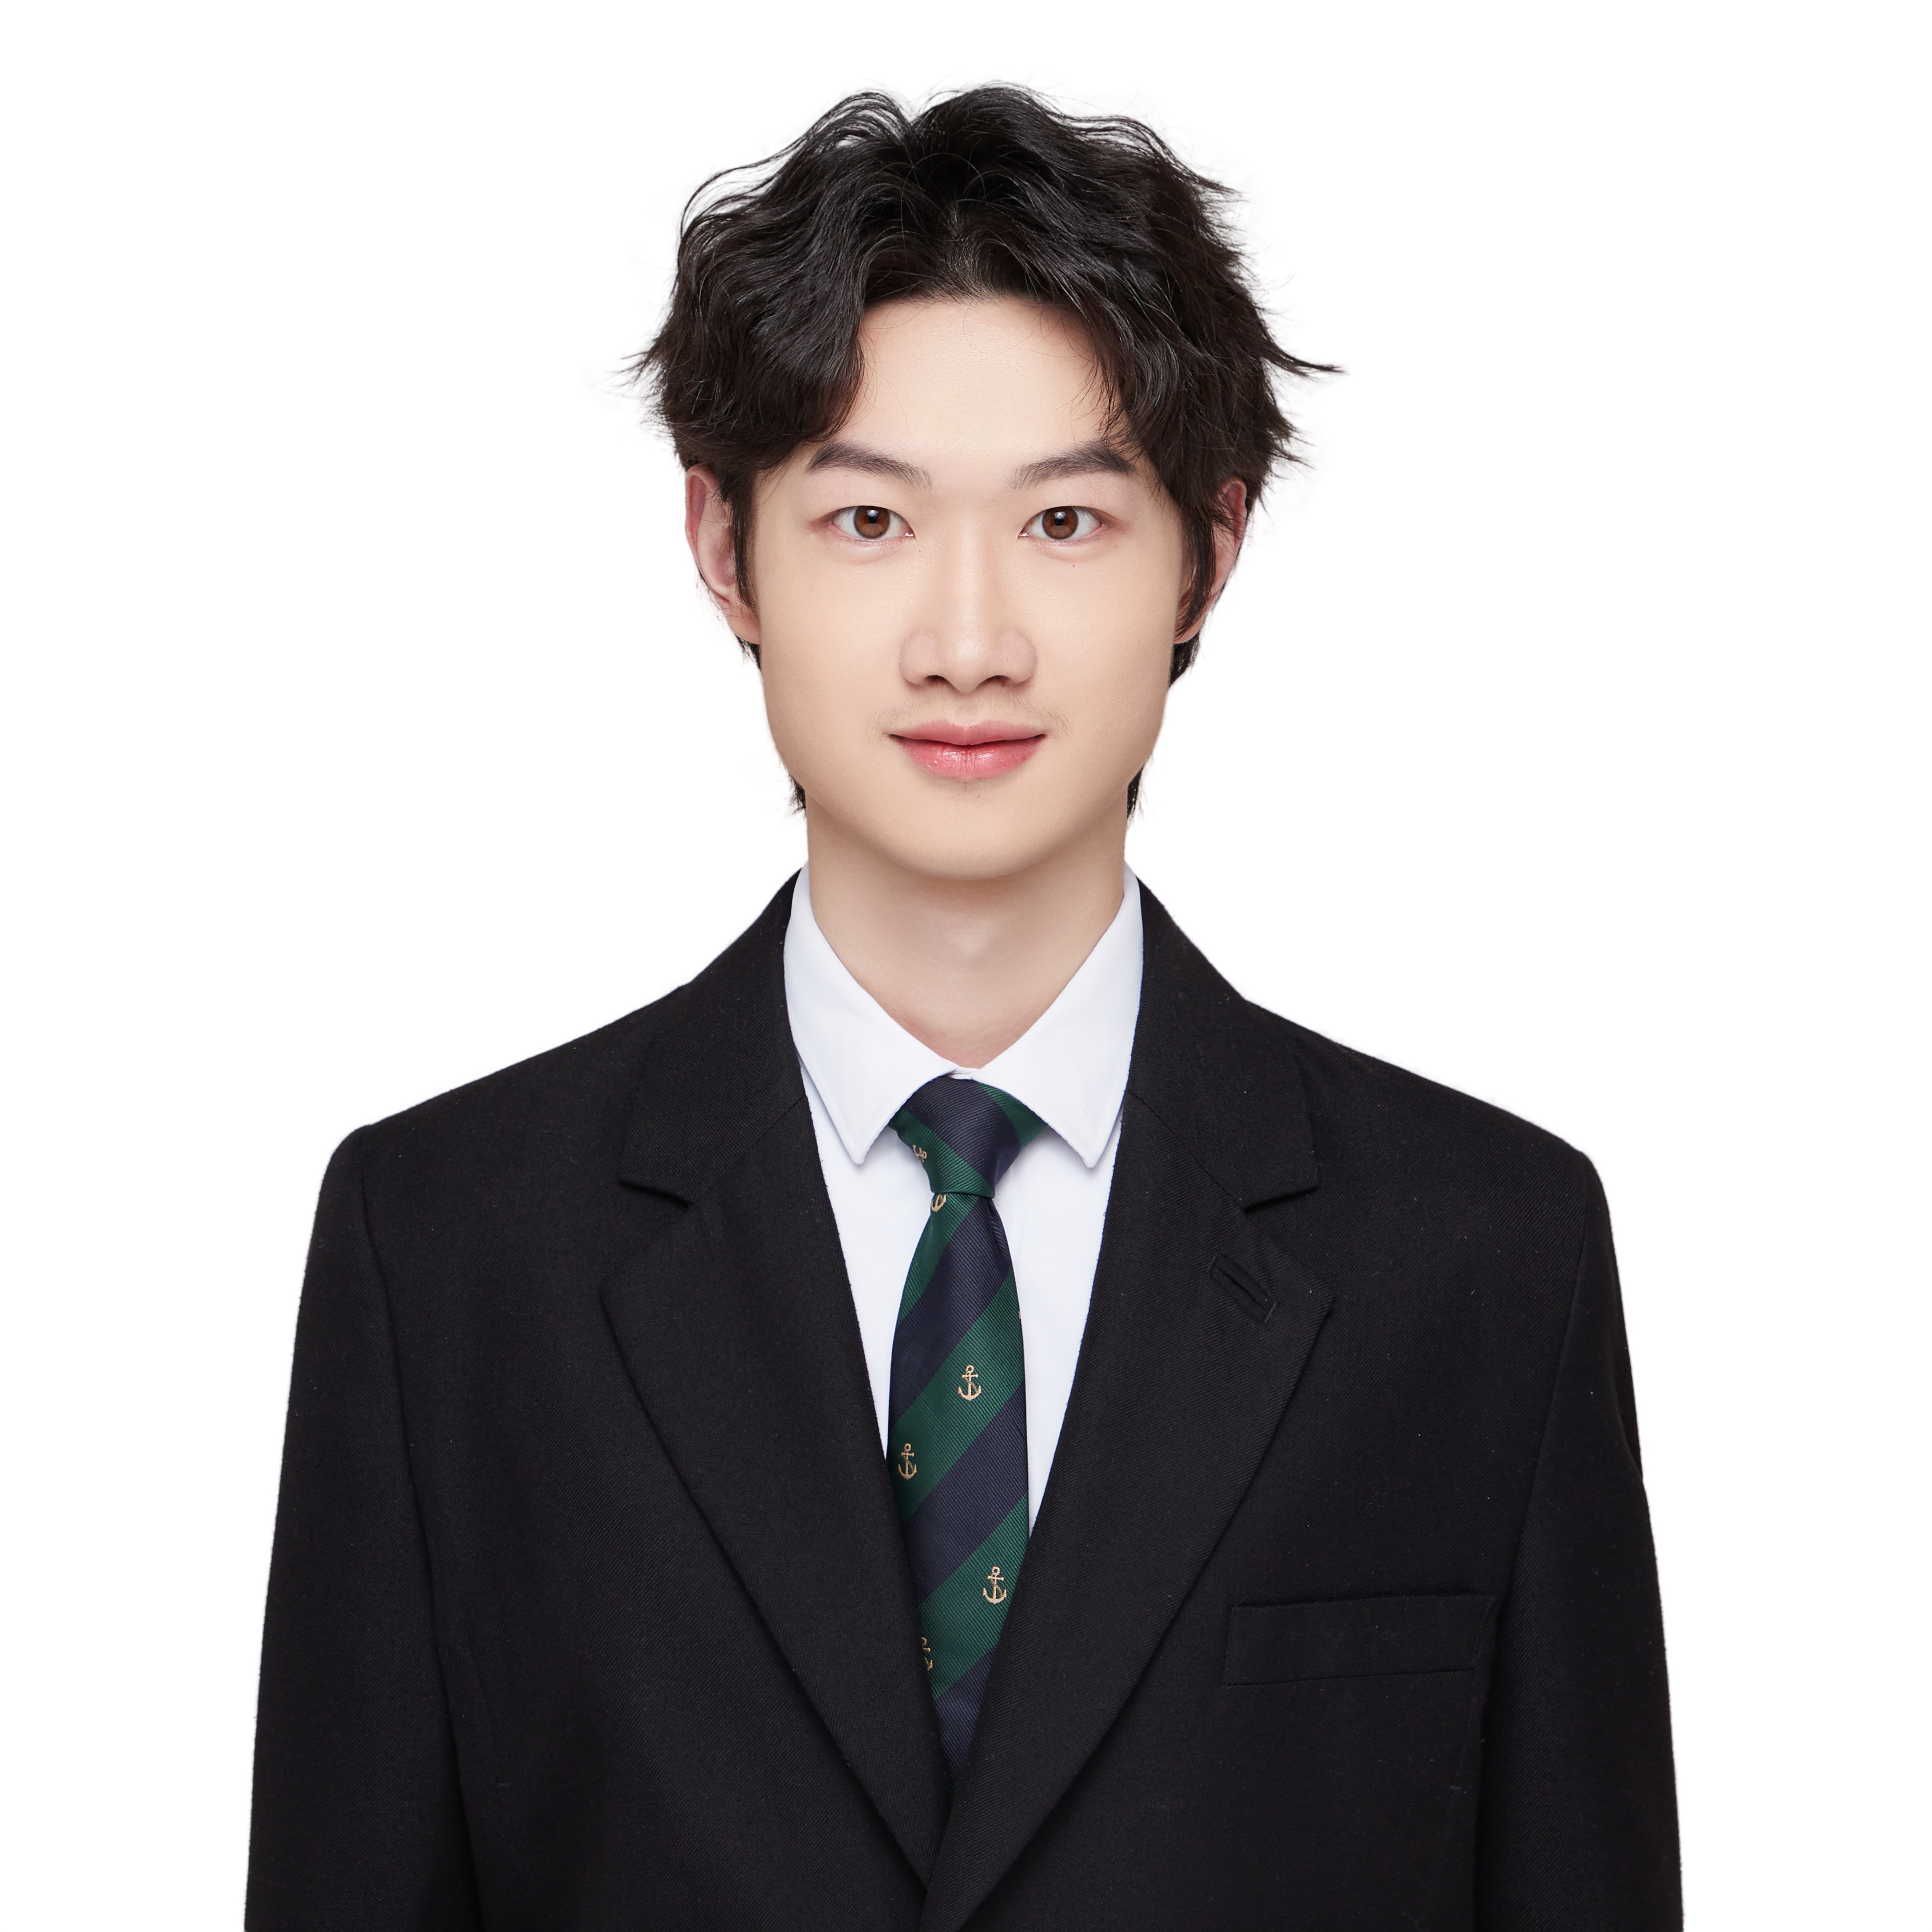
\includegraphics[width=0.88in]{pic.JPG}} & \scshape{Luyangyu Tong} & {Python~}\progressbar{0.75} \\
    & \email{lyytong@stu.cqu.edu.cn} & {\LaTeX~}\progressbar{0.8} \\
    & \phone{(+86) 180-9417-9352} & {MATLAB~}\progressbar{0.5} \\
    & \github[My Website]{https://supergrapee.github.io/} & {Markdown~}\progressbar{0.7}
  \end{tabu}
}
}

\section{\faCogs\ Expected Position}
\begin{itemize}[parsep=0.5ex]
\item \textbf{Top choice(if avaliable):} Head teacher of Electrical and ELectronics Department
\item Lecturer
\end{itemize}

\section{\faGraduationCap\ Education}
\datedsubsection{\textbf{University of Tokyo}, Tokyo, Japan}{2024 -- 2026}
\textit{Master} in Electrical Engineering and Information Systems(EEIS), matriculated in October 2024
\datedsubsection{\textbf{Chongqing University}, Chongqing, China}{2020 -- 2024}
\textit{B.S.} in Biomedical Engineering (BME) \quad GPA: 88/100 \quad Rank: Top 5\%

\section{\faUsers\ Related Experience}
\datedsubsection{\textbf{Application of IME Master's program in UTokyo}}{Jun. 2023 -- Feb. 2024}
\role{Offer}{Electrical Engineering and Information Systems}
Detailed application introduction link: \faChain \href{https://www.zhihu.com/question/443613502/answer/3247244151}{How I get admitted by the University of Tokyo?}.
\begin{itemize}
  \item \textbf{Receive the offer in Feb. 2024}
  \item Will study in the University of Tokyo from 2024 to 2026
  \item Admitted through the International Multidisciplinary Engineering(IME) program
\end{itemize}

\datedsubsection{\textbf{Teaching Assistant in Courses}}{Dec. 2021 -- Jun. 2022}
\role{Teaching Assistant}{Mathematical Modeling, ELectronics and Circuits, Physics}
Brief introduction: Working as an assistant in above courses to help students with their study.
\begin{itemize}
  \item My contribution includes: 
\begin{itemize}
  \item  Revising homework 
  \item  Making courseware
  \item  Monduting exercises 
  \item  Answering questions
\end{itemize} 
  \item \textbf{Excellent teaching assistant(Top 5\%)} during the semester
  \item Willing to get along with students
  \item More like a sincere friend than a serious teacher
\end{itemize}


% Reference Test
%\datedsubsection{\textbf{Paper Title\cite{zaharia2012resilient}}}{May. 2015}
%An xxx optimized for xxx\cite{verma2015large}
%\begin{itemize}
%  \item main contribution
%\end{itemize}

\section{\faHeartO\ Honors and Awards}
\datedline{\textit{\nth{2} Prize}, Award on National Mathematical Contest in Modeling }{Sep. 2022}
\datedline{\textit{\nth{2} Prize}, Award on National English Competition for College Students}{May. 2022}
\datedline{\textbf{\textit{Finalist}, Award on Mathematical Contest In Modeling (Top 0.17\% of all paper)}}{\textbf{May. 2022}}
\datedline{\textit{\nth{2} Prize}, Scholarship for Hongshen Honor College students(GPA Top 5\%)}{Dec. 2022}

\section{\faInfo\ Verbal Abilities}
\begin{itemize}[parsep=0.5ex]
  \item TOEFL: Overall 109(Speaking 24/Writing 27/Reading 29/Listening 29)
  \item GRE: Overall 319(Verbal 149/Quantitative 170/Analytical 3.5)
  \item CET-6 \& CET-4: 626 \& 610
  \item Still a Japanese learner\dots, expected to pass JLPT N2 in Sep. 2024.
\end{itemize}

%% Reference
%\newpage
%\bibliographystyle{IEEETran}
%\bibliography{mycite}
\end{document}
